\section{Network Programming}

\subsection{Terms and Networking Concepts}
Network programming refers to the practice of creating software that communicates over computer networks. Python provides several modules and libraries that facilitate network communication, making it relatively easy to develop networked applications.

\begin{itemize}
    \item \textbf{REST (Representational State Transfer)}\\
    REST is a style of software architecture for distributed systems, commonly used in networked applications like web services. It utilizes standard HTTP methods (GET, POST, PUT, DELETE) to manipulate resources, typically represented in formats such as JSON or XML. RESTful services follow principles such as statelessness, uniform interface, and resource-based interactions, making them scalable, flexible, and easily understandable.
    
    \item \textbf{Network Sockets}\\
    Network sockets are endpoints for communication between devices over a network. Sockets are used to establish connections and exchange data between a client and a server. They allow bidirectional data flow, enabling applications to send and receive data across networks using protocols such as TCP or UDP. Sockets provide an abstraction for handling network communication, allowing developers to create networked applications efficiently.
    
    \item \textbf{Protocols}\\
    Protocols are rules or standards that define how data is transmitted and received between devices on a network. They specify formats for data packets, error handling procedures, and other aspects of communication. Examples of network protocols include TCP/IP (Transmission Control Protocol/Internet Protocol), HTTP (Hypertext Transfer Protocol), and SMTP (Simple Mail Transfer Protocol).
    
    \item \textbf{Domains}\\
    Domains refer to the hierarchical naming system used to identify resources on the internet. They are part of the Domain Name System (DNS) and are used to assign memorable names to numerical IP addresses. For example, "google.com" is a domain name.
    
    \item \textbf{Addresses}\\
    Addresses are identifiers used to locate resources on a network, such as computers, servers, or other devices. In the context of the internet, addresses typically refer to IP addresses (Internet Protocol addresses), which are numerical labels assigned to each device connected to a computer network. For example, an IP address might be \texttt{192.0.2.1}.
    
    \item \textbf{Ports}\\
    Ports are virtual endpoints used by communication protocols to identify specific processes or services on a networked device. They allow multiple services or applications to operate concurrently on a single device. Ports are identified by numbers, and each service typically uses a specific port number. For example, web servers commonly use port 80 for HTTP and port 443 for HTTPS.
    
    \item \textbf{Services}\\
    Services refer to the software applications or processes running on a networked device that provide specific functions or features. These functions can include serving web pages, sending emails, transferring files, and more. Each service typically operates using one or more network protocols and may use specific ports for communication. Examples of services include web servers (e.g., Apache, Nginx), email servers (e.g., Microsoft Exchange, Postfix), and file transfer protocols (e.g., FTP, SFTP).
\end{itemize}

\newpage 
%\subsection{Network communication}

\subsubsection{Connection-oriented vs. Connectionless}
Network communication refers to the exchange of data between devices like computers, servers, routers, etc. over a network. This communication enables devices to share information, resources, and services. In networking, communication methods play a crucial role in determining how data is transmitted between devices. Two fundamental approaches are connection-oriented and connectionless communication. Connection-oriented communication establishes a dedicated link between sender and receiver for reliable data transfer, as seen in TCP. Conversely, connectionless communication, exemplified by UDP, sends independent packets without a prior connection, prioritizing speed over reliability.

\begin{itemize}
    \item \textbf{Connection-Oriented Communication:} In connection-oriented communication, a dedicated connection is established between the sender and receiver before any data transfer occurs. This connection remains active throughout the entire communication session. Protocols like TCP (Transmission Control Protocol) provide connection-oriented communication, ensuring reliable and ordered delivery of data.
    
    \item \textbf{Connectionless Communication:} In contrast, connectionless communication does not require a pre-established connection between the sender and receiver. Each data packet is sent independently and may take a different route to reach its destination. Protocols like UDP (User Datagram Protocol) operate in a connectionless manner. While connectionless communication is faster and more efficient for certain types of data, it may result in lost or out-of-order packets.
\end{itemize}

\subsubsection{Protocols: TCP and UDP}
A protocol is a set of rules or guidelines that govern how data is transmitted and received between devices, systems, or components in a networked environment. These rules define the format, timing, sequencing, and error handling of data transmission, ensuring that communication occurs in an organized, reliable, and efficient manner.\\

\begin{itemize}
    \item \textbf{Transmission Control Protocol (TCP)}
    \begin{itemize}
        \item Connection-oriented protocol
        \item Provides reliable, ordered, and error-checked delivery of data
        \item Uses acknowledgments and retransmissions for reliability
        \item Slower than UDP due to overhead of connection setup and error checking
        \item Suitable for applications requiring guaranteed delivery and data integrity, such as web browsing, email, and file transfer
    \end{itemize}

    \item \textbf{User Datagram Protocol (UDP)}
    \begin{itemize}
        \item Connectionless protocol
        \item Provides fast, but unreliable, delivery of data
        \item No guarantees on delivery, ordering, or duplicate protection
        \item Minimal overhead, making it faster than TCP
        \item Suitable for real-time applications, such as streaming media, online gaming, and VoIP, where speed is prioritized over reliability
    \end{itemize}
\end{itemize}

\newpage
\subsubsection{Clients and Servers}
In computer networking, clients and servers play integral roles in facilitating communication and accessing resources over a network. Clients, such as devices, programs, or processes, initiate requests for services or resources from servers.

\begin{itemize}
    \item \textbf{Clients:} Devices, programs, or processes that request services or resources from other devices or programs, known as servers. In a client-server model, clients initiate communication by sending requests to servers. These requests can vary widely depending on the type of service being requested. For example, a web browser acts as a client when it requests web pages from a web server, while an email client requests emails from an email server. Clients typically do not provide services directly to other devices or clients; instead, they rely on servers to fulfill their requests.
    
    \item \textbf{Servers:} Devices, programs, or processes that provide services, resources, or data to clients over a network. They listen for incoming requests from clients and respond by providing the requested services or resources. Servers can offer a wide range of services, including web hosting, email hosting, file storage, and database management. In a client-server model, servers are responsible for handling incoming requests from clients and delivering the appropriate responses. Unlike clients, servers do not typically initiate communication; instead, they wait for incoming requests from clients and respond accordingly.
\end{itemize}

The requests can vary depending on the service required, such as web pages or emails. Servers, on the other hand, respond to client requests by providing the requested services or resources. They listen for incoming requests and deliver appropriate responses, offering services like web hosting, email hosting, and file storage. Together, clients and servers form the foundation of the client-server model, enabling efficient communication and resource sharing across networks.\\

\begin{figure}[htbp]
    \centering
    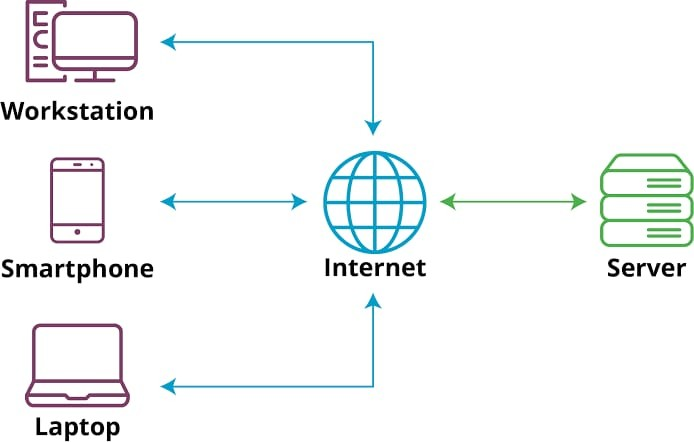
\includegraphics[width=0.7\textwidth]{images/client-server.jpg}
    \caption{Client server communication}
    \label{fig:example-np-2}
\end{figure}

\newpage
\subsection{Socket Programming}
Socket programming is a key aspect of network programming that enables communication between processes across a network. It forms the foundation for building various networked applications, allowing computers to exchange data over the internet or within a local network. In socket programming, a socket represents an endpoint for communication between two machines. A socket is an endpoint for communication between two machines. It consists of an IP address and a port number.
\begin{itemize}
    \item \textbf{IP Address:} An IP (Internet Protocol) address uniquely identifies a device on a network. In socket programming, IP addresses are used to establish connections between machines. An IP address is typically represented as a \textbf{32-bit number}, which is divided into four octets (each containing 8 bits) separated by periods. 
    \item \textbf{Port Number:} Port numbers are used to identify specific processes or services running on a machine. They facilitate multiplexing, allowing multiple applications to use the network simultaneously.
\end{itemize}

\begin{figure}[h!]
    \centering
    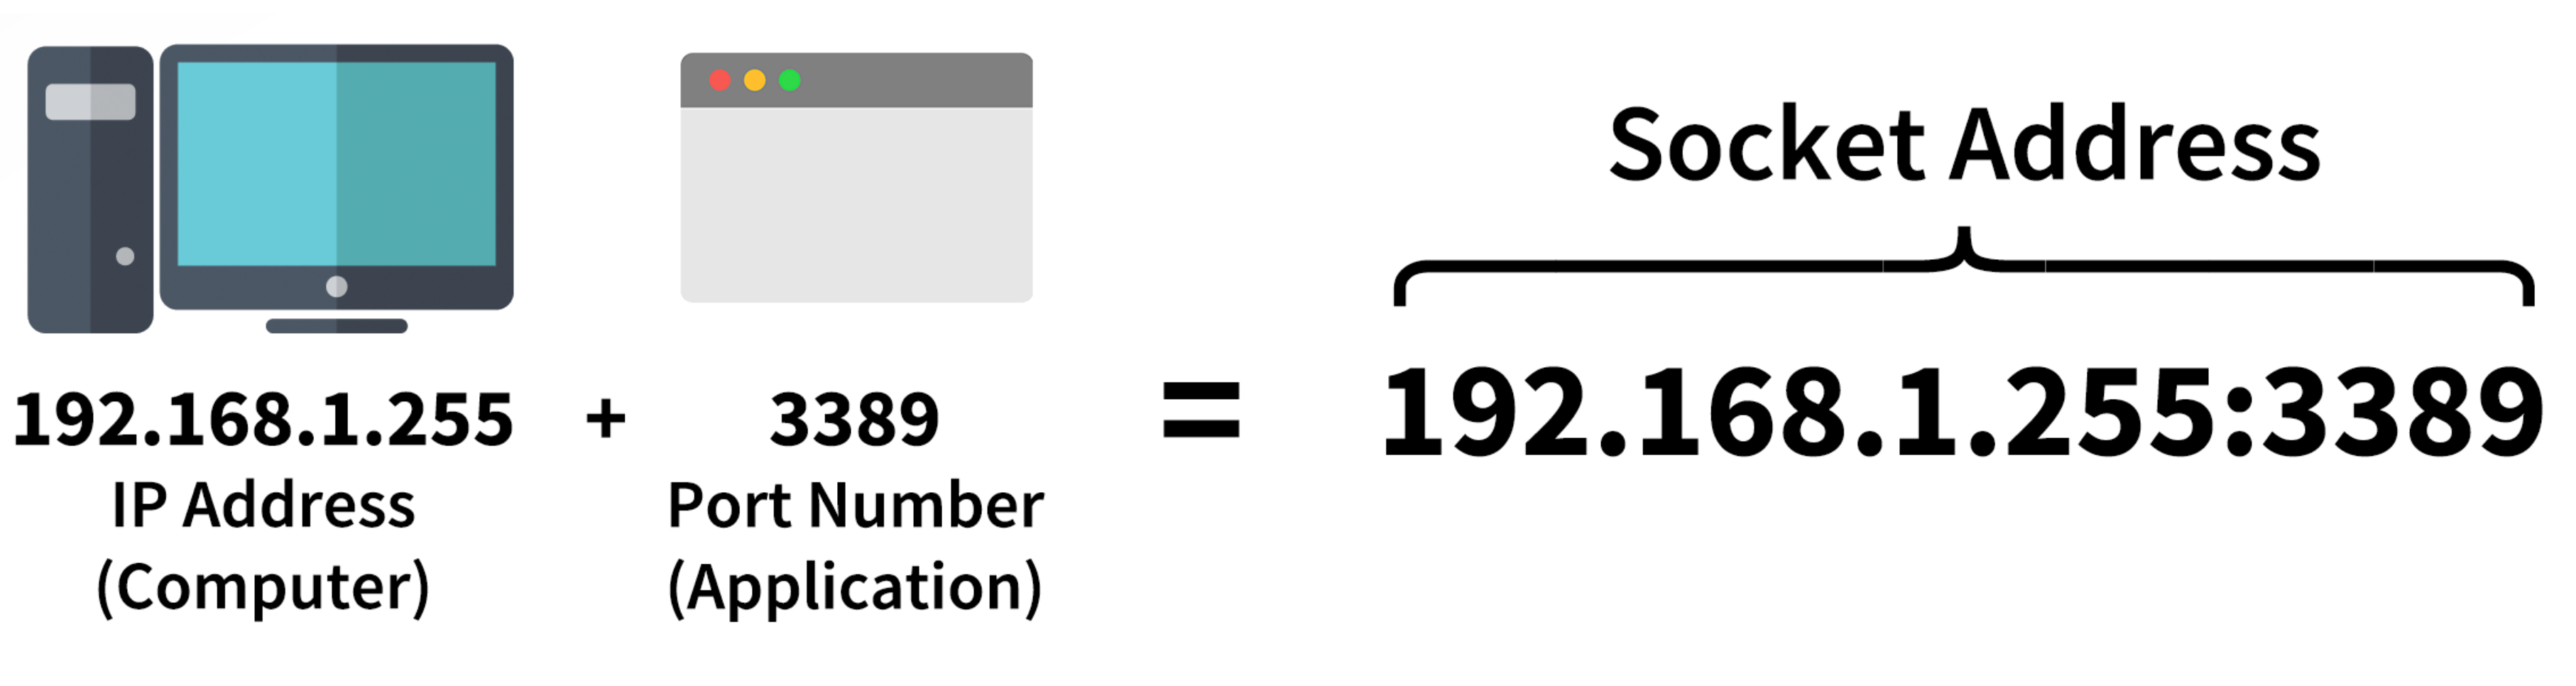
\includegraphics[width=0.6\textwidth]{images/socket_address.png}
    \caption{Socket address}
    \label{fig:example-np-1}
\end{figure}

\subsubsection{Types of Sockets}
\begin{itemize}[leftmargin=*]
    \item \textbf{Stream Sockets (TCP):} Stream sockets provide a reliable, connection-oriented communication channel. They ensure that data is delivered in the correct order without loss or duplication. TCP (Transmission Control Protocol) is commonly used for stream socket communication.
    \item \textbf{Datagram Sockets (UDP):} Datagram sockets provide an unreliable, connectionless communication channel. They allow for fast, low-overhead communication but do not guarantee delivery or order of messages. UDP (User Datagram Protocol) is commonly used for datagram socket communication.
\end{itemize}

\begin{codebox}
\begin{minted}{python}
import socket

# Creating a TCP socket
tcp_socket = socket.socket(socket.AF_INET, socket.SOCK_STREAM)

# Creating a UDP socket
udp_socket = socket.socket(socket.AF_INET, socket.SOCK_DGRAM)
\end{minted}
\end{codebox}

By specifying \texttt{socket.SOCK\_STREAM} for TCP and \texttt{socket.SOCK\_DGRAM} for UDP, the respective socket types are indicated to the \texttt{socket.socket()} function, allowing the creation of TCP or UDP sockets accordingly.

\newpage
\subsubsection{How Sockets Work}
\textbf{server.py}
\begin{codebox}
\begin{minted}{python}
import socket
import threading

SERVER = socket.gethostbyname(socket.gethostname()) # IP address of the server
PORT = 5050  # Port to listen on
ADDR = (SERVER, PORT)  # Address to bind the server
HEADER_SIZE = 64  # Size of the header containing message length
FORMAT = 'utf-8'  # Format to encode/decode messages
DISCONNECT_MSG = "!DISCONNECT"  # Message to disconnect a client

# Create a new socket
server = socket.socket(socket.AF_INET, socket.SOCK_STREAM)
server.bind(ADDR)

# Function to handle client connections
def handle_client(conn, addr):
    print(f"[NEW CONNECTION] {addr} connected")
    connected = True
    while connected:
        # Receive the header containing the message length
        header = conn.recv(HEADER_SIZE).decode(FORMAT)
        if header:
            msg_length = int(header)
            msg = conn.recv(msg_length).decode(FORMAT)
            if msg == DISCONNECT_MSG:
                connected = False
            print(f"[{addr}] {msg}")
            # Send acknowledgment to the client
            conn.send("[MESSAGE RECEIVED]".encode(FORMAT))
    conn.close()

# Function to start the server
def start():
    print(f"[LISTENING] server is listening on {SERVER}")
    server.listen()
    while True:
        # Wait for a new connection and store IP address and port
        conn, addr = server.accept()
        # Create a new thread to handle the client
        thread = threading.Thread(target=handle_client, args=(conn, addr))
        thread.start()
        print(f"[ACTIVE CONNECTIONS] {threading.active_count() - 1}")

if __name__ == "__main__":
    print("[STARTING] server is starting...")
    start()  # Start the server
\end{minted}
\end{codebox}

\newpage
\textbf{client.py}

\begin{codebox}
\begin{minted}{python}
import socket

# Get the IP address of the server dynamically
SERVER = socket.gethostbyname(socket.gethostname())
# Alternatively, specify IP address manually from ipconfig (IPv4 Address)
# SERVER = "192.168.12.30"
PORT = 5050  # Port on which the server is listening
ADDR = (SERVER, PORT)  # Address of the server
HEADER_SIZE = 64  # Size of the header containing message length
FORMAT = 'utf-8'  # Format to encode/decode messages
DISCONNECT_MSG = "!DISCONNECT"  # Message to disconnect from the server

# Create a new socket for the client
client = socket.socket(socket.AF_INET, socket.SOCK_STREAM)
client.connect(ADDR)

def send(message):
    # Encode the string message into bytes object
    message_encoded = message.encode(FORMAT)
    # Calculate the length of the encoded message
    message_length = str(len(message_encoded)).encode(FORMAT)
    # Pad the message length to ensure it matches HEADER_SIZE
    message_length += b' ' * (HEADER_SIZE - len(message_length))
    # Send the padded message length and the encoded message to the server
    client.send(message_length)
    client.send(message_encoded)

    # Receive messages from the server and print them
    print(client.recv(2048).decode(FORMAT))

# Send an initial message to the server
send("Hello, server!")

while True:
    # Continuously prompt the user for input
    msg = input("")

    if msg == "EXIT":
        # Send DISCONNECT_MSG to inform the server and break the loop
        send(DISCONNECT_MSG)
        break

    if msg:
        # If the user input is not empty, send it to the server
        send(msg)
\end{minted}
\end{codebox}

\newpage
\subsubsection{Connecting Sockets to HTTP Servers}
\begin{codebox}
\begin{minted}{python}
import socket

def send_http_request(host, port, request):
    # Create a socket object
    with socket.socket(socket.AF_INET, socket.SOCK_STREAM) as s:
        try:
            # Connect to the server
            s.connect((host, port))
            
            # Send the HTTP request
            s.sendall(request.encode())
            
            # Receive the response
            response = s.recv(4096)
            
            # Return the response
            return response.decode()
        
        except socket.error as e:
            print(f"Socket error: {e}")
        
        except Exception as e:
            print(f"An unexpected error occurred: {e}")
        
        finally:
            # Close the connection
            s.close()

# Example usage
if __name__ == "__main__":
    HOST = 'example.com'
    PORT = 80
    REQUEST = 'GET / HTTP/1.1\r\nHost: example.com\r\n\r\n'
    res = send_http_request(HOST, PORT, REQUEST)
    print(res)
\end{minted}
\end{codebox}

\begin{codebox}
\begin{minted}{python}
REQUEST = "GET / HTTP/1.1\r\nHost: www.example.com\r\n\r\n"
\end{minted}
\end{codebox}

This line is a string representing an HTTP request. It follows the HTTP protocol format:

\begin{itemize}
    \item \textbf{GET}: It's the HTTP method used to request data from a specified resource.
    \item \textbf{/}: It's the path of the resource being requested, in this case, it's the root path.
    \item \textbf{HTTP/1.1}: It specifies the version of the HTTP protocol being used.
    \item \textbf{\textbackslash r\textbackslash n}: It's a carriage return and line feed, used as a line break in HTTP requests.
    \item \textbf{Host: example.com}: It's a header specifying the domain name of the server.
    \item \textbf{\textbackslash r\textbackslash n}: Another line break.
    \item \textbf{\textbackslash r\textbackslash n}: An empty line indicating the end of the HTTP request headers.
\end{itemize}

\newpage
\subsubsection{Exceptions}
When working with Python sockets, which are used for network communication, there are several common exceptions. Handling these exceptions appropriately in your code ensures robustness and graceful error recovery during network communication.

\begin{itemize}
    \item \textbf{socket.error} or \textbf{socket.timeout}: These exceptions are the most general ones when working with sockets. They can occur for various reasons such as connection issues, timeouts, or other low-level socket errors.
    
    \item \textbf{ConnectionRefusedError}: This exception occurs when attempting to connect to a remote server that actively refuses the connection. It could indicate that the server is not running or is not accepting connections on the specified port.
    
    \item \textbf{ConnectionResetError}: This exception occurs when the connection is unexpectedly closed by the peer. It might happen due to network issues or if the peer terminates the connection unexpectedly.
    
    \item \textbf{BrokenPipeError}: This exception occurs when writing to a socket that has been closed at the other end. It typically happens when the connection is broken before all data has been sent or received.
    
    \item \textbf{TimeoutError}: This exception occurs when a socket operation times out. It can happen when attempting to establish a connection or during data transmission if there's no response within the specified timeout period.
    
    \item \textbf{OSError}: This is a general exception for various operating system-related errors. It can include errors related to file descriptors, permissions, or other low-level issues that might affect socket operations.
    
    \item \textbf{socket.gaierror}: This exception occurs when the address resolution fails. It could happen if the hostname cannot be resolved or if there's an issue with the network configuration.
    
    \item \textbf{socket.herror}: This exception occurs when a DNS-related error happens. It might occur when the DNS server is unreachable or if there's an issue with the hostname.
    
    \item \textbf{BlockingIOError}: This exception occurs when an operation would block if the \texttt{socket} is in non-blocking mode. It usually happens during non-blocking socket operations.
    
    \item \textbf{PermissionError}: This exception occurs when there's a permission-related issue, such as trying to bind to a privileged port without sufficient permissions.
\end{itemize}


\newpage
\subsection{REST Clients}
A REST (Representational State Transfer) client is a program or module that sends HTTP requests to a RESTful web service or API to interact with resources on the server. REST is an architectural style for designing networked applications, commonly used in web services development.

There are several libraries and frameworks available for creating REST clients. One popular choice is the \texttt{requests} library, which provides a simple and elegant way to send HTTP requests and handle responses.

\subsubsection{The \texttt{requests} Module}
The \texttt{requests} module simplifies the process of working with HTTP requests and responses, making it an essential tool for web scraping, web development, and interacting with web APIs.

\begin{codebox}
\begin{minted}{python}
import requests

# Making a GET request to the XKCD website
r = requests.get('https://xkcd.com/353/')

# Printing the available attributes and methods of the response object 'r'
#print(dir(r))

# Printing the help documentation for the response object 'r'
#print(help(r))

# Making a GET request to download the image from the XKCD website
img = requests.get('https://imgs.xkcd.com/comics/python.png')

# Printing the content of the image (binary data)
print(img.content)

# Printing the status code of the image request
print(img.status_code)

# If the response from the XKCD website is successful
if r.ok:
    # If response is ok, open a file named 'comic.png' in binary write mode
    with open('comic.png', 'wb') as f:
        # Write the binary content of the image to the file
        f.write(img.content)
\end{minted}
\end{codebox}

\newpage
\subsubsection{CRUD Operations}
CRUD is an acronym that stands for Create, Read, Update, and Delete. It represents the four basic operations that can be performed on data stored in a database or managed by an application:

\begin{itemize}
    \item \textbf{Create}: This operation involves adding new data or records to the database. In a database context, it typically means inserting a new row into a table. In an application context, it could involve creating new objects or entities.
    
    \item \textbf{Read}: This operation involves retrieving existing data or records from the database. In a database context, it typically means querying the database to retrieve specific data based on certain criteria. In an application context, it could involve fetching and displaying data to the user.
    
    \item \textbf{Update}: This operation involves modifying existing data or records in the database. In a database context, it typically means updating the values of one or more columns in a specific row. In an application context, it could involve allowing users to edit and update information.
    
    \item \textbf{Delete}: This operation involves removing existing data or records from the database. In a database context, it typically means deleting a row from a table. In an application context, it could involve allowing users to delete objects or entities.
\end{itemize}

CRUD operations form the foundation of many applications and are commonly used in various software systems, including web applications, mobile apps, and desktop applications. These operations allow users to interact with and manage data effectively, enabling applications to create, retrieve, update, and delete information as needed.

\subsubsection{HTTP Methods: GET, POST, PUT, DELETE}

HTTP (Hypertext Transfer Protocol) methods define the actions that a client (such as a web browser) can perform on a server. Each HTTP method is associated with a specific type of action that the client wants to perform on a resource identified by a URL.

\begin{itemize}
    \item \textbf{GET}: Used to retrieve data from a server, such as fetching a web page or an image.
    
    \item \textbf{POST}: Used for submitting data, uploading files, or making changes to a server's state.
    
    \item \textbf{PUT}: Used to update existing resources with new data.
    
    \item \textbf{DELETE}: Used to delete resources from a server, such as deleting a user account or a file.
\end{itemize}

\newpage
\begin{codebox}
\begin{minted}{python}
import requests

# Target URL for HTTP requests: https://httpbin.org/

# GET request with parameters passed directly in the URL
# r = requests.get('https://httpbin.org/get?page=2&count=25') # errorprone

# GET request with params
params = {'page':2, 'count': 25}
r = requests.get('https://httpbin.org/get', params=params)
print(r.url)
print(r.text)

# POST request with form data
form_data = {'username': 'corey', 'password': 'testing'}
r = requests.post('https://httpbin.org/post', data=form_data)
print(r.text)
r_dict = r.json()
print(r_dict['form'])

# GET request with Basic Authentication
auth = ('corey', 'testing')
r = requests.get('https://httpbin.org/basic-auth/corey/testing', auth=auth)
print(r)
print(r.text)

# Example of setting a timeout for a request
r = requests.get('https://httpbin.org/delay/1', timeout=2)
print(r)

# Example causing a timeout
r = requests.get('https://httpbin.org/delay/5', timeout=3)
print(r)
\end{minted}
\end{codebox}

\newpage
\subsubsection{Response Status Codes}
Response status codes are standardized three-digit integers that HTTP servers use to communicate the outcome of a client's request. They provide information about whether a request was successful, encountered an error, or requires further action. The status code is accompanied by a short, human-readable phrase that provides additional context. HTTP status codes are grouped into five categories, each represented by the first digit of the status code.

\begin{itemize}
    \item \textbf{1xx - Informational:}
    \begin{itemize}
        \item Request has been received and understood, and that further action is required by the client.
    \end{itemize}
    
    \item \textbf{2xx - Success:}
    \begin{itemize}
        \item \textbf{200 OK:} The request was successful.
        \item \textbf{201 Created:} The request has been fulfilled, and a new resource has been created.
        \item \textbf{204 No Content:} Request has been successfully processed by the server, but it is not returning any content.
    \end{itemize}
    
    \item \textbf{3xx - Redirection:}
    \begin{itemize}
        \item Further action is needed by the client to fulfill the request. They typically indicate that the client should take additional steps to complete the request.
    \end{itemize}
    
    \item \textbf{4xx - Client Error:}
    \begin{itemize}
        \item \textbf{400 Bad Request:} Server cannot process the request due to a client error, like invalid syntax.
        \item \textbf{401 Unauthorized:} Request requires authentication, but the client has not provided valid credentials.
        \item \textbf{404 Not Found:} Server cannot find the requested resource.
    \end{itemize}
    
    \item \textbf{5xx - Server Error:}
    \begin{itemize}
        \item \textbf{500 Internal Server Error:} Server encountered an unexpected condition that prevented it from fulfilling the request.
    \end{itemize}
\end{itemize}




Response status codes are essential for understanding the outcome of HTTP requests and diagnosing issues with web applications and APIs. By interpreting these status codes, clients can respond appropriately to the Server's response and handle errors or redirections effectively.

\newpage
\subsubsection{Analyzing the Server's Response}
Analyzing a server's response with the \texttt{requests} library involves examining various attributes of the response object returned by the requests module after making an HTTP request. Here's a basic overview of how to analyze a server's response using requests:

\begin{codebox}
\begin{minted}{python}
import requests

# Send a GET request
response = requests.get('https://api.example.com/data')

# Print the status code
print('Status Code:', response.status_code)

# Print the response headers
print('Headers:', response.headers)

# Print the response content as text
print('Response Text:', response.text)

# Print the URL of the response
print('URL:', response.url)

# Print any cookies sent by the server
print('Cookies:', response.cookies)

# Convert response content to JSON (if applicable)
try:
    json_data = response.json()
    print('Response JSON:', json_data)
except ValueError:
    print('Response is not in JSON format')

# Print time elapsed between sending the request and receiving the response
print('Elapsed Time:', response.elapsed.total_seconds(), 'seconds')
\end{minted}
\end{codebox}
